
\subsection{PID Parameter Training}












\subsection{Object Grasping}
\jgonote{Including open and closed loop paradigms, learning specific and generic grasp models.}

We consider a setting where a robotic arm
with 7 degrees of freedom grasps objects with a parallel plate gripper which adds
an additional degree of freedom, but much of what we discuss could be extended to other
arms and grippers, for instance the universal jamming gripper ~\citep{}.

We use a dual rate PID controller in the sense that we use two sets of PID coefficients. The
first set is for making large adjustments when the aim if off by a significant amount. The
second set is for making small adjustments when aim is close to the target.

Our system is distributed and thus at times there is an appreciable amount of latency between
communicating components. Care is taken to synchronize robot movement with object detection
reports, allowing only a fixed amount of movement per report.

Visual servoing tutorial paper: \citep{chaumette06}

\begin{figure*}
  \begin{center}
    \begin{tabular}{l c}
      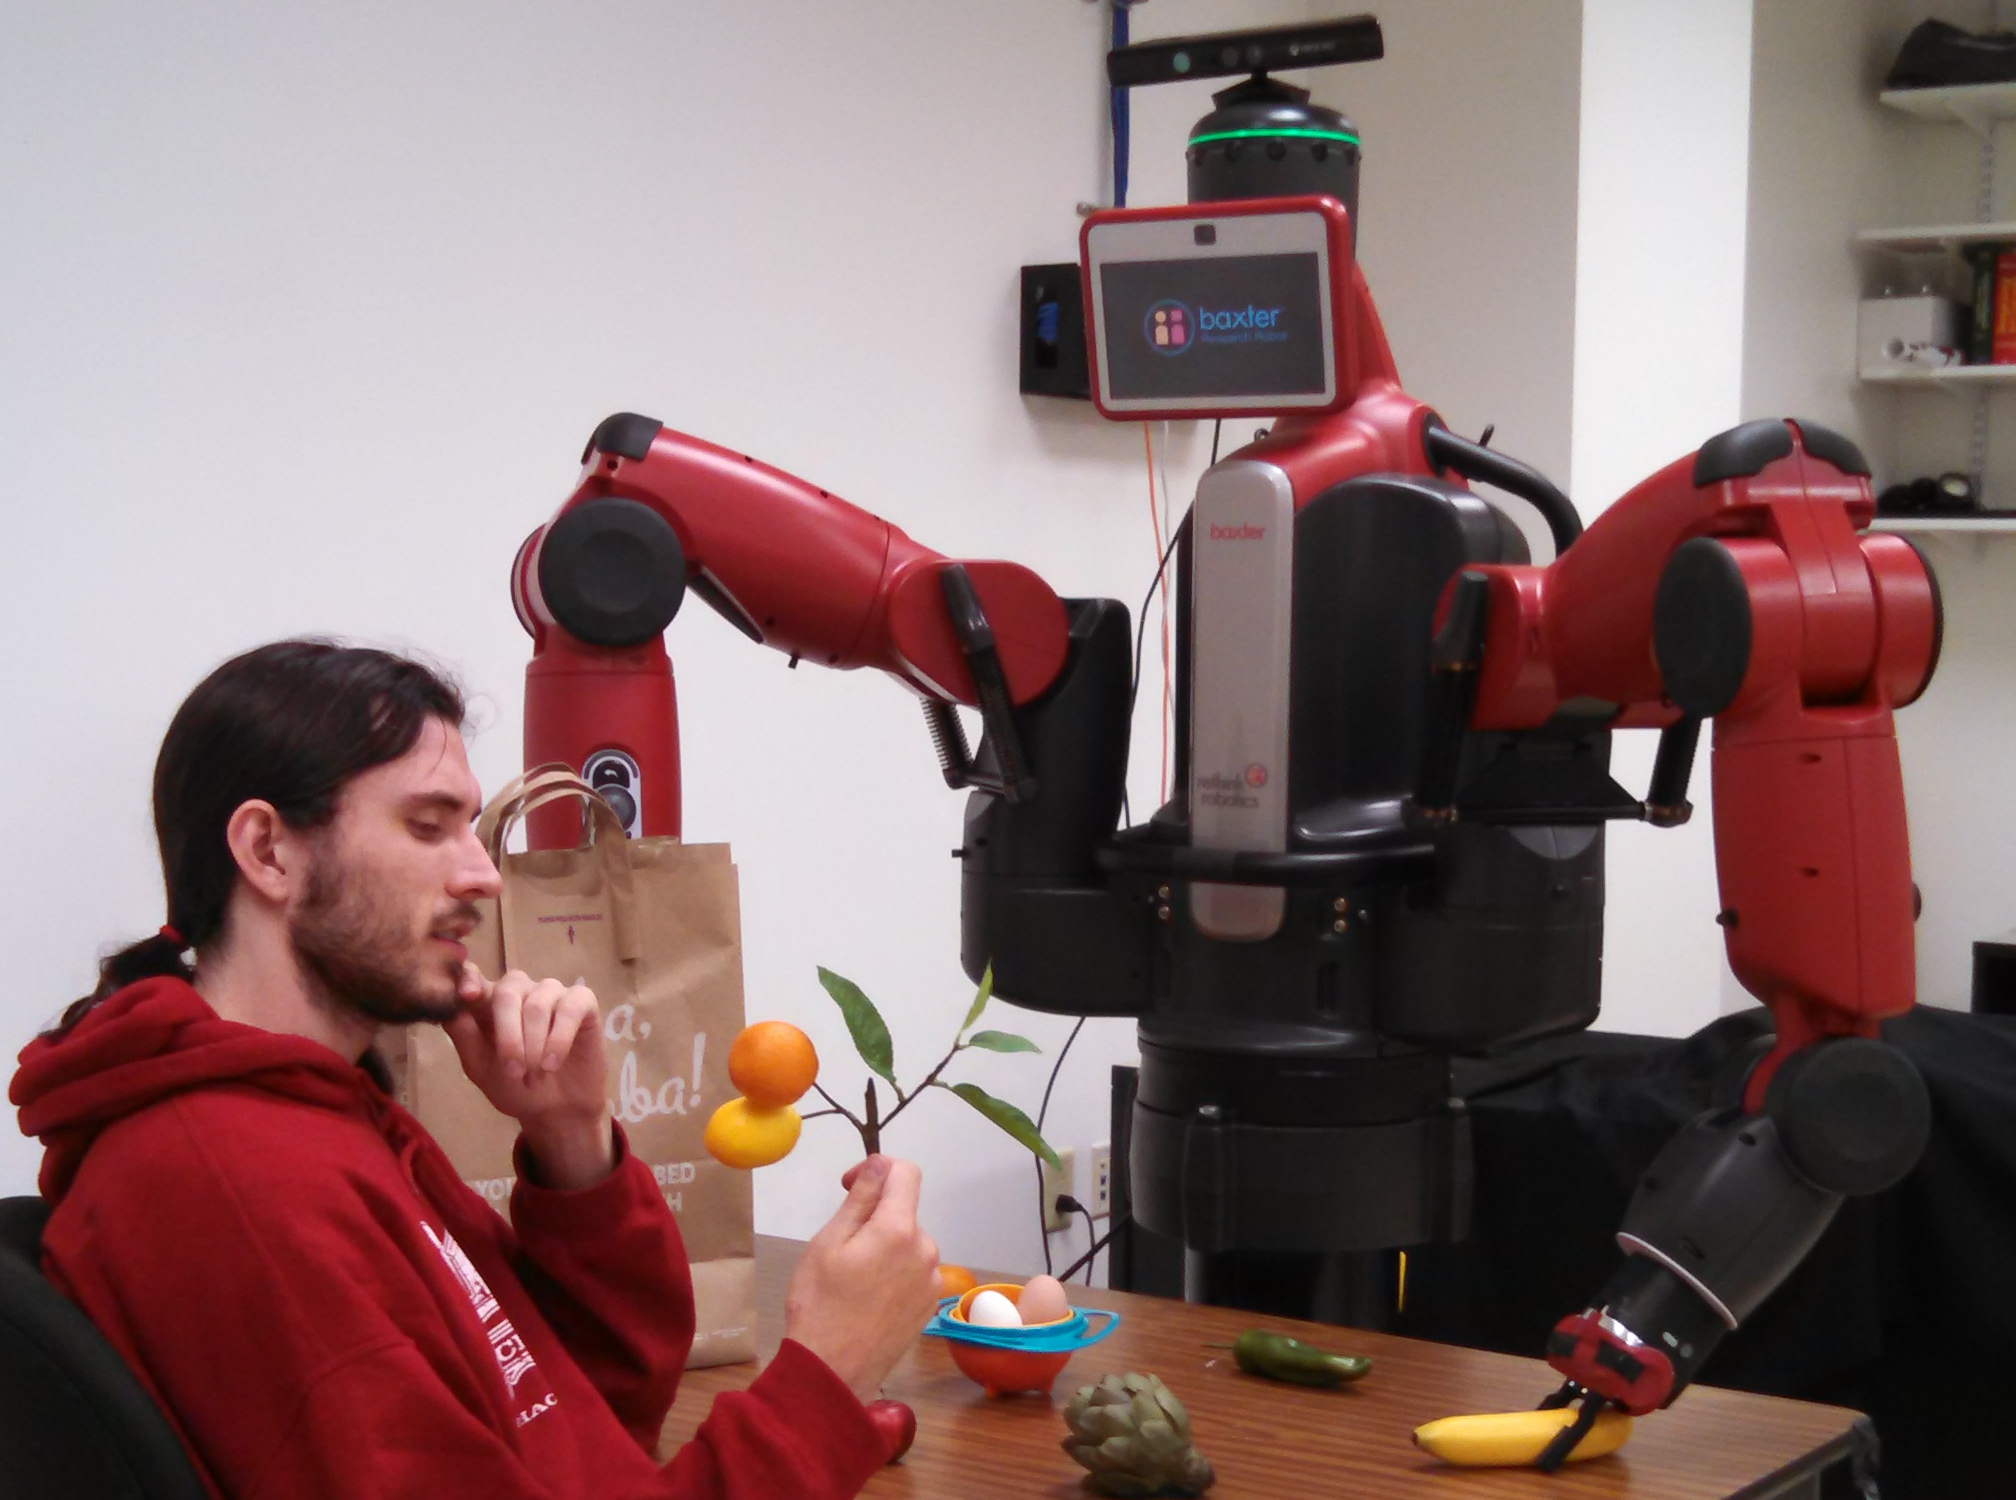
\includegraphics[width=200px, height=150px]{robo2.png} &
      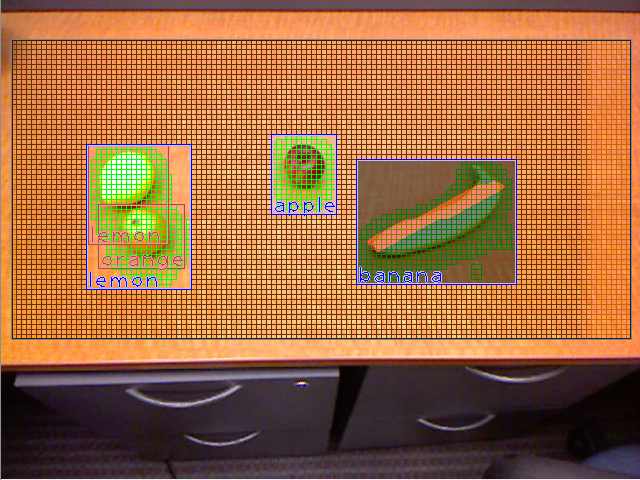
\includegraphics[width=200px, height=150px]{screen2.png} \\
    \end{tabular}
  \end{center}
  \caption{Left: Baxter uses visual servoing to grasp an object. Right: The view through Baxter's wrist camera, 
    showing the location of the target as well as the objective reticle.}
\end{figure*}

\stnote{Cite the visual servoing tutorial paper and talk about the
  connection to grasping rectangles.}

This Grasp Rectangle business fits in nicely with the reticle.

0. Estimate the depth of the table by inspecting non-object locations. This helps decide when to close the gripper.

1. Servo orientation to the '0' orientation, or one of a few sparsely sampled keypoint orientations.
Each viewing orientation (from the wrist) is tied to a grasping orientation.

2. Servo to a 'normal' scale. This is fixed, we don't want multiple scales running around.

3. Now instead of aiming at the center, aim at a proposed target offset from the center.


\subsection{PID Controller}
\jgonote{Maybe a coordinate descent algorithm or wide-scale random noise search.}
Since we use a dual-rate controller, there are two separate sets of coefficients that we must train.
We train the high-rate coefficients with the objective of getting the aim within the ``close'' threshold.
We train the low-rate coefficients with the objective of getting the aim within the 'hit' threshold.
The training for the high and low-rate coefficients is analogous and happens independently, so
without loss of generality we describe the training process for an arbitrary set of coefficients.

\jgonote{I imagine this has been done before so it would be good to find who did this.}
\stnote{Find someone to learn PID coefficients.}
A single set of PID coefficients consists of $K_P$, $K_I$, $K_D$. In the inside loop of EM-like training, we
randomly pick a coefficient $K$ to train, fix the other two coefficients,  and use a local search 
algorithm ~\citep{} to find the optimal value of $K$ conditioned on the fixed values of the other two
parameters. This problem is not necessarily convex and so we run the inside loop of our algorithm
until we have converged to a local minimum.


\section{Simultaneous Localization and Mapping of Tabletop Objects}

We aim to autonomously acquire instance-based models of objects based
on exploration.  To carry out this inference, we follow approaches
based on recursive state estimation~\citep{thrun08} and
SLAM~\citep{durrant06}.  In our approach, the map that the robot is
acquiring is not an occupancy grid or landmark locations, as in
conventional SLAM, but rather knowledge of the appearance and grasp
points of the objects being mapped.  The localization problem is
estimating the pose of these objects at each time step.  We can also
jointly estimate the pose of the robot's end effector, but this pose
is often known with high accuracy in the local coordinate system.  The
graphical model for our approach appears in Figure~\ref{fig:model}.

\begin{figure}
\centering
\includegraphics{model-crop.pdf}
\caption{Graphical model for our proposed approach.\label{fig:model}}
\end{figure}

We define the following variables:
\begin{itemize}
\item $x_t = \left< r_t, o_1 \dots o_k \right>$.  Our state consists of
  the pose of the robot's end effector, $r_t$, along with the pose and
  category of all the objects currently being tracked, $o_1 \dots o_k$.
\item $z_t = \left<r, g, b, d\right>$.  Our observation consists of
  the pixel values and depth generated from a sensor on the robot's
  end effector.  This sensor could be a depth camera from the Kinect;
  in our experiments we use a one-pixel depth camera created from
  Baxter's IR sensor and wrist camera.
\item $u_t = \left\{\left<x, y, z, r, p, y\right>\right.$ Alternately,
  the robot could attempt to grasp the object, leading to a new
  configuration of objects in the workspace.
\item $m$ The map consists of a colored voxel map for each object. 
\end{itemize}

We aim to jointly estimate a distribution over object poses along with
the map, $m$:
\begin{align}
p(x_t, m |  z_0 \dots z_t, u_0 \dots u_t)
\end{align}

We formulate this problem as a Bayes' filter with a time update:
\begin{align}
p&(x_t, m | z_0 \dots z_{t-1}, u_0 \dots u_t) = \notag\\
&\int p(x_t | x_{t-1}, u_t) \times p(x_{t-1}, m | z_{0} \dots z_{t-1}, u_{0} \dots u_{t-1}) dx_{t-1}
\end{align}

and a measurement update: 
\begin{align}
p(&x_t, m | z_0 \dots z_t, u_0 \dots u_t) = \notag\\
&\frac{p(z_t | x_t, m) P(x_t, m | z_0 \dots z_{t-1}, u_0 \dots u_t)}
{p(z_t | z_{0} \dots z_{t-1}, u_0 \dots u_t)}
\end{align}

\subsection{Transition Model}

Our transition model incorporates the effect of the control input on
the robot's end effector as well as on all the objects:
\begin{align}
p(x_t | x_{t-1}, u_t) &= p(r_t, o^1_t \dots o^k_t | r_{t-1}, o^1_{t-1} \dots o^k_{t-1}, u_t) \\
\intertext{We assume that the robot's end effector pose and the object poses are independent:}
                     &= p(r_t | u_t) \times p(o^1_t \dots o^k_t | o^1_{t-1} \dots o^k_{t-1}, u_t)
\intertext{
We also assume that each object is independent of the
others; although in general we would like the robot to predict the
effects of its grasps, in practice other objects can be moved by
mistake.  Therefore our transition model will have high uncertainty
over all objects when the robot moves any object.}
                    &\approx p(r_t | u_t) \times \prod_k p(o^k_t | o^k_{t-1}, r_t)
\end{align}

We endow the robot with two types of control actions.  In the first
type, the robot plans collision free motions with conservative models
of the boundaries of possible objects; these types of transitions move
the robot's end effector but leave all the object poses unchanged.
The second type is when the robot grasps an object.  After an
attempted grasp we assume the pose of all the objects have moved and
need to be reestimated (in case the robot knocked an object during its
attempted grasp)

\subsection{Measurement Model}

Our sensor consists of a depth camera; for simplicity we update one
pixel at a time, although a sensor such as the Kinect would consist of
many updates at once.
\begin{align}
p(z_t | x_t, m) = p(z_t | r_t, o_t^1 \dots o_t^k, m)
%
\intertext{When the object pose and map is known, we can identify the
  one object penetrated by the sensor:}
%
p(z_t | x_t, m) = p(z_t | r_t, o_t^i, m^i)
\end{align}

We assume a sensor model with Gaussian noise on pixel values and depth
values.

\subsection{Inference}

We carry out inference in the model using a Rao-Blackwellized Particle
Filter~\citep{durrant06}.  In particular we partition our state space
according to the product rule:

\begin{align}
p(&x_0 \dots x_t, m | z_0 \dots z_t, u_0 \dots u_t) = \notag\\
& p(m | x_0 \dots x_t, z_0 \dots z_t) \times p(x_0 \dots x_t | z_0 \dots z_t, u_0 \dots u_t)
\end{align}

Thus each particle is represented by the set:
\begin{align}
\left\{ w_t^{(i)}, x_0^{(i)} \dots x_t^{(i)}, p(m | x_0^{(i)} \dots x_t^{(i)}, z_0 \dots z_t)\right\}
\end{align}

In a simplified model, we can compute a maximum likelihood map
analytically from the pose and observation history, rather than
representing a distribution over it.

Our proposal distribution is the motion model, as in Fast Slam
1.0~\citep{montemerlo02}:
\begin{align}
x_t^{(i)} \sim  p(x_t | x_{t-1}^{(i)}, u_t)
\end{align}

That is, when objects do not move, we assume a fixed pose, together
with small random movement to correct initial pose estimation error.



\section{Applications of GRATA}

\subsection{Recognition Training}

\subsection{Pose Estimation Training}

\subsection{Grasp Training}
4. Once aiming is complete, save the image in the reticle, try to grasp, and save whether that grasp completed.
This can be ascertained by the gripper position.

5. Calculate a density map for this 



\subsection{GRATA Simulation}
Understanding the behavior of GRATA requires running the system many times. This would be impractical
to do on the actual robot. It is necessary use a simulator for the process so that we can dramatically shorten the
experimental iteration time. A dense sampling strategy is a good baseline and the data collected can
be queried by an active learning technique to simulate the process of data collection.

Using a dense sampling strategy, we approximate the set $D$ and can then run offline experiments using other
sampling strategies. However, the numbers we report are on actual executions of the system where
the robot gathers the data online.




\section{General Robotic Autonomous Training Algorithm}
\label{sec:training}
We teach the system by finding its weaknesses and training it to overcome them.

Our framework structures the training in a way that scales. 

When the robot asks for help, we can ground ambiguous object examples to the right class
and retrain the models online.

\subsection{GRATA Definition}

In the following algorithm design pattern, 
$X$ is the set of ground truth labels for the specified problem,
$Y$ is the set of all possible observations for the specified problem,
\mbox{$D \subset X \times Y$} is the set of all possible training pairs observable in our problem instance,
\mbox{$\{T_i\}_{i \in \mathbb{N}}$} is a sequence of curated sets of training examples (where \mbox{$\forall i \in \mathbb{N}, T_i \subset D$}),  
$\mathcal{T}$ is the power set of $D$,
\mbox{$O: \mathcal{T} \to \mathbb{R}$} is the objective function that we are trying to optimize 
(which includes the implementation of the physical actions the robot must take to evaluate it),
\mbox{$S: \mathbb{N} \to \mathbb{R}$} is the objective function history (i.e. \mbox{$S(i) = O(T_i)$}),
$\mathcal{S}$ is the set of all possible objective function histories,
\mbox{$H: \mathcal{S} \times \mathbb{N} \to \{0,1\}$} is a function which decides whether to ask for help at
a specified time step,
\mbox{$\mathcal{C} = \mathcal{T} \times \mathcal{S} \times \mathbb{N}$} is the complete training state,
\mbox{$G: \mathcal{C}$} is a function which implements asking for and receiving help (e.g. auditing and grounding data under bad conditions
or asking for a new collections strategy or a crucial example),
\mbox{$P: \mathcal{C} \to \{0,1\}$} is a function that evaluates a stopping criterion and decides whether to continue training,
and \mbox{$L: \mathcal{C} \to D$} a function that proposes a new ground truth $x \in X$ and collects a corresponding observation $y \in Y$ to form
a new training example \mbox{$(x,y) = d \in D$}. 

\begin{table}
  \begin{center}
  \caption{The list of symbols we use in the definition of GRATA.}
  \begin{tabular}{lr}
    \toprule
    Symbol & Meaning \\ 
    \midrule
    $X$  & Ground Truth Labels \\
    $Y$  & Observations \\
    $D \subset X \times Y$  & Universe of Observable Data \\
    $\{T_i\}_{i \in \mathbb{N}}$  & Sequence of Training Sets \\
    $\mathcal{T} = 2^D$ & All Possible Training Sets \\
    $O: \mathcal{T} \to \mathbb{R}$ & Objective Function \\
    $S: \mathbb{N} \to \mathbb{R}$  & Objective Function History \\
    $\mathcal{S} = \{S: \mathbb{N} \to \mathbb{R}\}$  & All Possible Objective Function Histories \\
    $H: \mathcal{S} \times \mathbb{N} \to \{0,1\}$  & Help Criterion \\
    $\mathcal{C} = \mathcal{T} \times \mathcal{S} \times \mathbb{N}$  & Complete Training Set \\
    $G: \mathcal{C}$  & Help Request \\
    $P: \mathcal{C} \to \{0,1\}$  & Stopping Criterion \\
    $L: \mathcal{C} \to D$  & Sample Proposal \\
  \bottomrule
  \end{tabular}
  \end{center}
\end{table}



Applying GRATA to a problem involves defining the above quantities and implementing the high level algorithm
in the figure ~\citep{}.

\begin{figure}
  \textbf{GRATA}
  \begin{algorithmic}
  \STATE $t\gets 1$
  \STATE $c\gets 1$
  \STATE $T_1 = \emptyset$
  \STATE $S(1)\gets 0$
  \STATE $i\gets 1$
  \WHILE{$c$}
    \IF {$H(S,i) == 1$}
      \STATE $G(T_i, S,i)$
    \ELSE
      \STATE $d\gets L(T_i, S, i)$
      \STATE $T_{i+1}\gets T_i \cup \{d\}$
    \ENDIF
    \STATE $i\gets i+1$
    \STATE $S(i)\gets O(T_i)$
    \STATE $c\gets P(T_i, S, i)$
  \ENDWHILE
  \end{algorithmic}
  \caption{The high-level generalized robotic automatic training algorithm (GRATA) which we employ.}
\end{figure}



\jgonote{Computer vision approaches, geometry and point cloud based approaches. Dieter Fox's automatic
training pipeline (how well developed is it? we may need to sell our approach as being a 
general algorithm for allowing a robot to train arbitrary subsystems in order to differentiate 
ourselves.)}



%% We tackle the pose estimation problem using the same
%% classification pipeline that we use for object recognition. We train a
%% separate pose classifier for each object class. This time, the class
%% assigned to each training example is the orientation from which the
%% object is viewed in that example.  During inference, we first
%% determine the object class of a candidate bounding box, and once the
%% class is known we apply the corresponding pose classifier to determine
%% the orientation from which we are viewing the object. We combine this
%% orientation with position information from the point cloud information
%% derived from the D channel of the RGB-D video to form a full pose
%% estimate.
